\begin{knitrout}
\definecolor{shadecolor}{rgb}{0.969, 0.969, 0.969}\color{fgcolor}\begin{figure}

{\centering 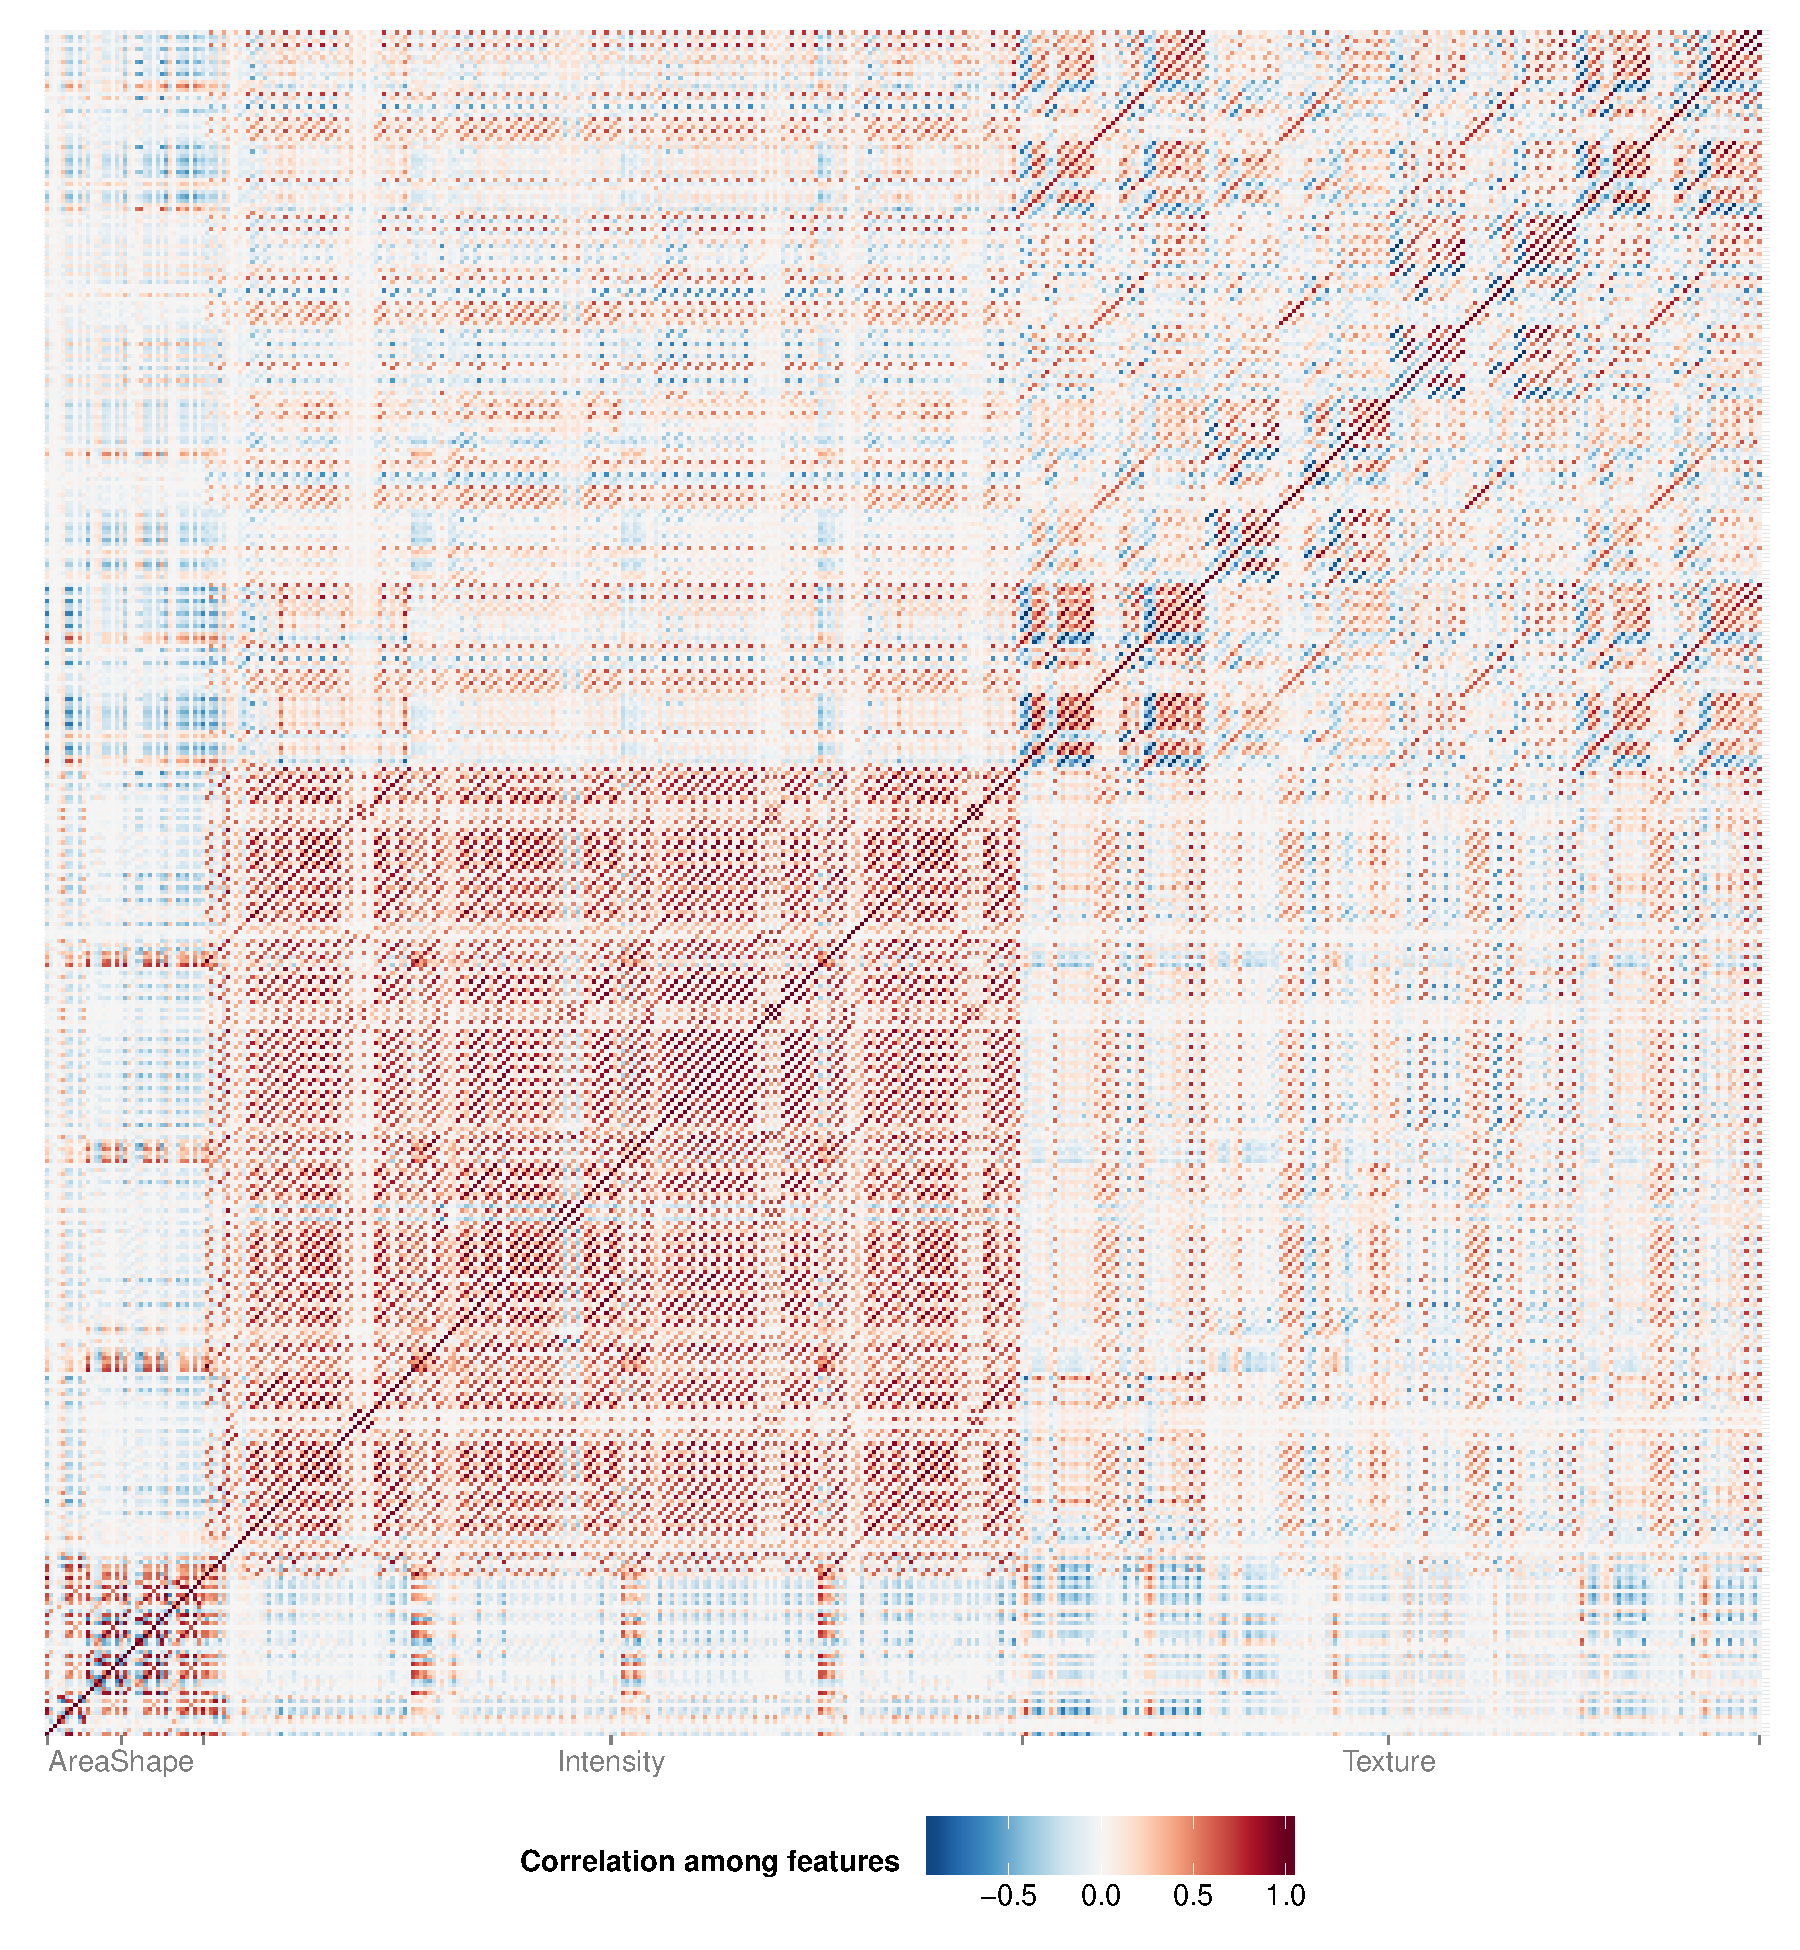
\includegraphics[width=\maxwidth]{figures/R/correlation-heatmap-analysis-correlation-1} 

}

\caption[Heatmap representation of correlation among single cell features.]{A heatmap representation of the correlation matrix obtained by sampling 10\% of single cell feature data available for plate J110-2D illustrates severe correlation among many features that is typical for all datasets. This comes as no surprise due to the redundancy in measured features. The three diagonal blocks correspond to three groups of features, \textit{AreaShape}, \textit{Intensity} and \textit{Texture}.}\label{fig:analysis-correlation}
\end{figure}


\end{knitrout}

